
\chapter{Examples of {\ADAPTSYSTEM}}
\label{ch:adapt-example}


\section{Two Round Odd Elements}
\label{sec:adapt-example-tr-odd}
We present a variant of the previous two round example in Figure~\ref{fig:tworound_odd}. In this odd example, only the data at odd index of the database is used.
%
{
\begin{figure}
\begin{subfigure}{.4\textwidth}
\begin{centering}
$\begin{array}{l}
    % \left[j \leftarrow 0 \right]^1 ; \\
   \clabel{ \assign{a}{0}  }^{1} ; \\
    \clabel{\assign{j}{0} }^{2} ; \\
    \eloop ~ \clabel{3}^{3} ~ \edo ~ \\
   \quad 
     \eif ( \clabel{( j \% 2 == 0)}^{4}\\
     \quad \quad ,\clabel{ \assign{x}{ q(\chi[j+1])} }^{5}  \\
     \quad \quad ,\clabel{\assign{x}{ q(\chi[j]) }}^{6} ) ;\\
     \quad \clabel{\assign{a}{ a+x} }^{7}  ;\\
     \quad \clabel{ \assign{j}{j+1} }^{8}      ;\\
 \clabel{l \leftarrow q(a*\chi[3]) }^{9}\\
\end{array} $
\caption{}
\end{centering}
\end{subfigure}
\begin{subfigure}{0.5\textwidth}
\begin{centering}
$
\begin{array}{l}
    \clabel{ \assign{a_1}{0}  }^{1} ; \\
    \clabel{\assign{j_1}{0} }^{2} ; \\
    \eloop ~ \clabel{3}^{3} , 0,  ~ \edo ~ [(j_3, j_1,j_2), (a_3, a_1,a_2)], \\
  \quad 
     \eif ( \clabel{( j_3 \% 2 == 0)}^{4}, [x_3,x_1,x_2], [],[]\\
     \quad \quad ,\clabel{ \assign{x_1}{ q(\chi[j_3+1])} }^{5}  \\
     \quad \quad ,\clabel{\assign{x_2}{ q(\chi[j_3]) }}^{6} ) ;\\
     \quad \clabel{\assign{a_2}{ a_3+x_3} }^{7}  ;\\
     \quad \clabel{ \assign{j_2}{j_3+1} }^{8}      ;\\
 \clabel{l_1 \leftarrow q(a_3*\chi[3]) }^{9}\\
\end{array}$
\caption{}
\end{centering}
\end{subfigure}
    \vspace{-0.2cm}
    \caption{(a) The two round odd algorithm in labeled {\tt Loop} language, (b) The SSA program for the same example. }
    \label{fig:tworound_odd}
    \vspace{-0.5cm}
\end{figure}
}
%
This algorithm only touches the odd part of the database, by adding an extra if statement to checking the index $j$ in Figure~\ref{fig:tworound_odd}(a). The extra complexity is added to handle the newly generated variables in the loop and if statement in the SSA version in Figure~\ref{fig:tworound_odd}(b). 
The query-based dependency graph does not change a lot compared to the previous two rounds example in Figure~\ref{fig:simpl-two-round-graph}(c), but the node does change according to the trace. We assume $a = n$ in the final memory is the result of the sum of previous query results in the loop.
We give the trace $t = [q(\chi[1])^{5,[3:1]}, q(\chi[1])^{6,[3:2]}, q(\chi[3])^{5,[3:3]}, q(n* \chi[3])^{9,\emptyset} ]$ and use $q_1$ for $q(\chi[1])$, $q_3$ representing for $q(\chi[3])$, $q_4$ for $q(n* \chi[3])$. The query-based dependency graph based on this trace is shown in Figure~\ref{fig:odd_graphs}(a). We show the red path, which is a sequence of adaptively chosen queries of length $2$. So among the total $4$ queries, we have 2-round adaptive queries. According to Theorem~\ref{thm:gaussiannoise} and Theorem~\ref{thm:gaussiannoise2}, we will have a tighter upper bound on the generalization error if we know the adaptivity $2$, obtained from the red path in Figure~\ref{fig:odd_graphs}(a). 

Our algorithm {\ADAPTSYSTEM} gives us the upper bound on the aforementioned adaptivity $2$. We construct the variable-based weighted dependency graph in Figure~\ref{fig:odd_graphs}(b). The weighted nodes are in the red dashed circle and the red dashed paths show the most weighted path in the graph, with the weight $2$. So, for this two rounds odd algorithm, our system gives a tight upper bound $2$, which can be used to get a better generalization error bound.




\begin{figure}
    \begin{subfigure}{0.4\textwidth}
    \begin{centering}
    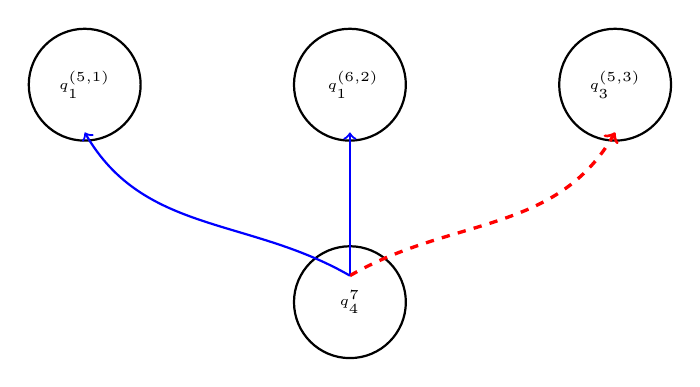
\begin{tikzpicture}[scale=\textwidth/18cm,samples=200]
%%% The nodes represents the k query in the first round
% \draw[very thick] (-1,6)  -- (13,6) -- (13,3) -- (-1,3) -- (-1,6);
% \draw[black] (-2.5, 4) circle (0pt) node [anchor=south]{\textbf{line 4:}};
\draw[thick] (1, 4.1) circle (30pt) node
% node[label={above: \small{iteration 1:}}] 
{\tiny{$q_1^{(5,1)}$}} ;
\draw[thick] (6, 4.1) circle (30pt) node
{\tiny{ $q_1^{(6,2)}$}};
 \draw[thick] (11, 4.1) circle (30pt) node 
{\tiny{$q_3^{(5,3)}$}};
% \filldraw[black] (-2.5, 0) circle (0pt) node [anchor=south]{\textbf{line 7:}};
\draw[thick] (6, 0) circle (30pt) node {\tiny{$q_4^7$}};
\draw[ thick,->, blue] (6, 0.5)  -- (6, 3.2) ;
\draw[very thick,->, red, dashed] (6, 0.5)  to [out=30,in=240] (11, 3.2) ;
\draw[ thick,->, blue] (6, 0.5)  to [out=150,in=300]  (1, 3.2) ;
\end{tikzpicture}
\caption{}
    \end{centering}
    \end{subfigure}
    \begin{subfigure}{0.5\textwidth}
    \begin{centering}
    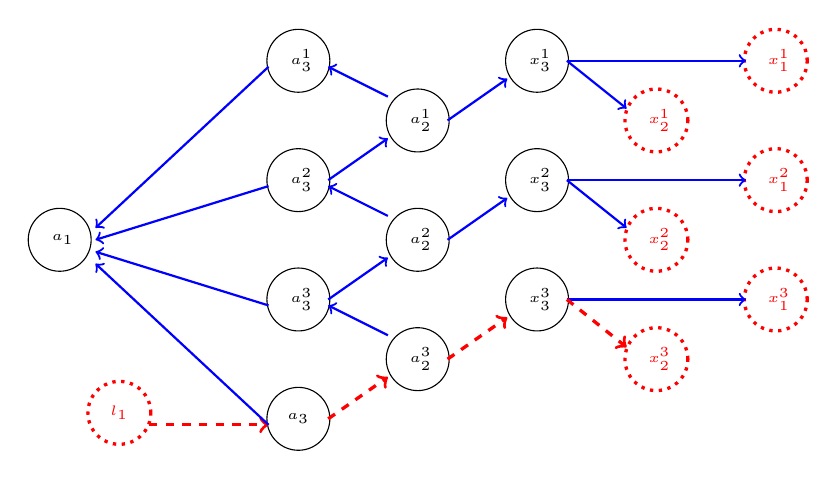
\begin{tikzpicture}[scale=\textwidth/16cm,samples=200]
%%% The nodes represents the k query in the first round
% \draw[very thick] (-1,6)  -- (13,6) -- (13,3) -- (-1,3) -- (-1,6);
% \draw[black] (-2.5, 4) circle (0pt) node [anchor=south]{\textbf{line 4:}};
% \draw[thick] (1, 1.1) circle (25pt) node
% % node[label={above: \small{iteration 1:}}] 
% {\tiny{$q_1^{(5,1)}$}} ;
\draw[] (2, 5.1) circle (15pt) node
{\tiny{ $a_1$}};
\draw[] (6, 8.1) circle (15pt) node
{\tiny{ $a_3^{1}$}};
\draw[very thick, red, dotted] (14, 8.1) circle (15pt) node
{\tiny{ $x_{1}^{1}$}};
\draw[very thick, red, dotted] (12, 7.1) circle (15pt) node
{\tiny{ $x_{2}^{1}$}};
\draw[] (10, 8.1) circle (15pt) node
{\tiny{ $x_{3}^{1}$}};
\draw[] (8, 7.1) circle (15pt) node
{\tiny{ $a_{2}^{1}$}};
\draw[] (6, 6.1) circle (15pt) node
{\tiny{ $a_3^{2}$}};
\draw[very thick, red, dotted] (14, 6.1) circle (15pt) node
{\tiny{ $x_{1}^{2}$}};
\draw[very thick, red, dotted] (12, 5.1) circle (15pt) node
{\tiny{ $x_{2}^{2}$}};
\draw[] (10, 6.1) circle (15pt) node
{\tiny{ $x_{3}^{2}$}};
\draw[] (8, 5.1) circle (15pt) node
{\tiny{ $a_{2}^{2}$}};
\draw[very thick, red, dotted] (14, 4.1) circle (15pt) node
{\tiny{ $x_1^{3}$}};
\draw[] (6, 4.1) circle (15pt) node
{\tiny{ $a_3^{3}$}};
\draw[] (10, 4.1) circle (15pt) node
{\tiny{ $x_3^{3}$}};
\draw[very thick, red, dotted] (12, 3.1) circle (15pt) node
{\tiny{ $x_2^{3}$}};
\draw[] (8, 3.1) circle (15pt) node
{\tiny{ $a_{2}^{3}$}};
 \draw[] (6, 2.1) circle (15pt) node 
{\tiny{$a_3$}};
% \filldraw[black] (-2.5, 0) circle (0pt) node [anchor=south]{\textbf{line 7:}};
\draw[very thick, red, dotted] (3, 2.2) circle (15pt) node {\tiny{$l_1$}};
 \draw[very thick,->, red, dashed] (3.5, 2)  -- (5.5, 2) ;
 \draw[very thick,->, red, dashed] (6.5, 2.1)  -- (7.5, 2.8) ;
 \draw[very thick,->, red, dashed] (8.5, 3.1)  -- (9.5, 3.8) ;
 \draw[thick,->, blue] (10.5, 4.1)  -- (13.5, 4.1) ;
  \draw[very thick,->, red, dashed] (10.5, 4.1)  -- (11.5, 3.3) ;
   \draw[thick,->, blue] (7.5, 3.5)  -- (6.5, 4.0) ;
   \draw[thick,->, blue] (6.5, 4.1)  -- (7.5, 4.8) ;
    \draw[thick,->, blue] (8.5, 5.1)  -- (9.5, 5.8) ;
     \draw[thick,->, blue] (10.5, 6.1)  -- (11.5, 5.3) ;
\draw[thick,->, blue] (10.5, 6.1)  -- (13.5, 6.1) ;
\draw[thick,->, blue] (7.5, 5.5)  -- (6.5, 6.0) ;
\draw[thick,->, blue] (6.5, 6.1)  -- (7.5, 6.8) ;
\draw[thick,->, blue] (8.5, 7.1)  -- (9.5, 7.8) ;
\draw[thick,->, blue] (10.5, 8.1)  -- (11.5 , 7.3) ;
\draw[thick,->, blue] (10.5, 8.1)  -- (13.5 , 8.1) ;
% \draw[thick,->, blue] (8.5, 9.1)  -- (9.5 , 9.8) ;
% \draw[thick,->, blue] (8, 9.6)  -- (8, 10.6) ;
\draw[thick,->, blue] (7.5, 7.5)  -- (6.5, 8.0) ;
\draw[thick,->, blue] (5.5, 8.0)  -- (2.6, 5.3) ;
\draw[thick,->, blue] (5.5, 6.0)  -- (2.6, 5.1) ;
\draw[thick,->, blue] (5.5, 4.0)  -- (2.6, 4.9) ;
\draw[thick,->, blue] (5.5, 2.0)  -- (2.6, 4.7) ;
% \draw[very thick,->, red] (6, 0.5)  to [out=30,in=240] (11, 3.2) ;
% \draw[very thick,->, blue] (6, 0.5)  to [out=150,in=300]  (1, 3.2) ;
\end{tikzpicture}
    \caption{}
    \end{centering}
    \end{subfigure}
    \vspace{-0.3cm}
    \caption{(a) The query-based dependency graph for odd example (b) The SSA variable-based weighted dependency graph for the same example, the node in red dashed circle is weighted.}
    \label{fig:odd_graphs}
    \vspace{-0.3cm}
\end{figure}
%
%
\section{ Multiple Round Algorithm}
\label{sec:adapt-example-mr}

%
The two round strategy works well in our framework, we explore further to look at an advanced adaptive data analysis algorithm - multiple round algorithm.
%
%
{\small
\begin{figure}
    \begin{subfigure}{0.35\textwidth}
    \begin{centering}
    $
    \begin{array}{l}
    %  \left[j \leftarrow 0 \right]^1 ; \\
    \clabel{I \leftarrow [] }^1; \\
    \clabel{\assign{ns}{0} }^{2}; \\
     \clabel{\assign{cs}{0} }^{3}; \\
    \eloop ~ [3]^{4} ~  
    \ ~ \edo ~ \\ 
    \quad \clabel{a \leftarrow q(f( I)) }^{5}; \\
    \quad \clabel{\assign{ns}{update\_nscore(a)}; }^{6}\\
    \quad \clabel{\assign{cs}{update\_cscore(a)}; }^{7}\\
    \quad \clabel{I \leftarrow \mathsf{update} ( I, ns, cs)  }^{8}
\end{array}
    $
    \caption{}
    \end{centering}
    \end{subfigure}
    \begin{subfigure}{0.4\textwidth}
    \begin{centering}
    $
    \begin{array}{l}
    %  \left[j \leftarrow 0 \right]^1 ; \\
    \clabel{I_1 \leftarrow [] }^1; \\
    \clabel{\assign{ns_1}{0} }^{2}; \\
     \clabel{\assign{cs_1}{0} }^{3}; \\
    \eloop ~ [3]^{4} , 0 ,  
     ~ \edo ~ [(I_3, I_1,I_2),(ns_3, ns_1,ns_2),(cs_3, cs_1,cs_2) ] \\ 
    \quad \clabel{a_1 \leftarrow q(f(I_3)) }^{5}; \\
   \quad \clabel{\assign{ns_2}{update\_nscore(a_1)}; }^{6}\\
   \quad \clabel{\assign{cs_2}{update\_cscore(a_1)}; }^{7}\\
   \quad \clabel{I_2 \leftarrow \mathsf{update} (I_3, ns_3, cs_3)  }^{8}
\end{array}
   $
   \caption{}
    \end{centering}
    \end{subfigure}
    \caption{(a) The labeled program implementing the multiple round algorithm (b)The same program in the SSA version.}
    \label{fig:multi_code}
    \end{figure}
}
%
%
% \[
%
% %
%
% %
% MR^{ssa}(k) \triangleq
% \begin{array}{l}
%     %  \left[j \leftarrow 0 \right]^1 ; \\
%     \left[I_1 \leftarrow [] \right]^1; \\
%     \eloop ~ [k]^{2} , 0, [I_3,I_1,I_2] \\ 
%     \ ~ \edo ~ \\ \Big(
%     \left[p_1 \leftarrow c \right]^3 ; \\
%     \left[ a_1 \leftarrow q (p, I_3) \right]^4;\\
%     \left[I_2 \leftarrow \mathrel{\mathsf{update}} ( {I_3}, (a_1, p_1))  \right]^5
%     \Big) 
% \end{array}
% \]
%
% \begin{algorithm}
% \footnotesize
% \caption{A multi-round analyst strategy for random data (Algorithm 5 in ...)}
% \label{alg:multiRound}
% \begin{algorithmic}
% \REQUIRE Mechanism $\mathcal{M}$ with a hidden state $X\in [N]^{n}$ sampled u.a.r., control set size $c$
% \STATE Define control dataset $C = \{0,1, \cdots, c - 1\}$
% \STATE Initialize $Nscore(i) = 0$ for $i \in [N]$, $I = \emptyset$ and $Cscore(C(i)) = 0$ for $i \in [c]$
% \STATE  {\bf for}\ $j\in [k]$\ {\bf do} 
% \STATE \qquad {\bf let} $p=\uniform(0,1)$ 
% \STATE \qquad {\bf define} $q (x) = \bernoulli ( p )$ .
% \STATE \qquad {\bf define} $qc (x) = \bernoulli ( p )$ .
% \STATE \qquad {\bf let} $a = \mathcal{M}(q)$ 
% \STATE \qquad {\bf for}\ $i \in [N]$\ {\bf do}
% \STATE \qquad \qquad $Nscore(i) = Nscore(i) + (a - p)*(q (i) - p)$ if $i \notin I$
% \STATE \qquad {\bf for}\ $i \in [c]$\ {\bf do}
% \STATE \qquad \qquad $Cscore(C(i)) = Cscore(C(i)) + (a - p)*(qc (i) - p)$
% \STATE \qquad {\bf let} $I = \{i | i\in [N] \land Nscore(i) > \max(Cscore)\}$
% \STATE \qquad {\bf let} $X = X \setminus I$ 
% \RETURN $X$.
% % \ENSURE 
% \end{algorithmic}
% \end{algorithm}
% %
%   We have seen the two round algorithm in Section~\ref{subsec:loop-syntax}. We show the multiple-round algorithm, which is an advanced algorithm.
%  \\
%
The multiple rounds algorithm starts from an initialized empty tracking list $I$, two scores called Nscore $ns=0$ and Cscore $cs=0$, initialzied to $0$. It goes $k$ rounds and at every round, the two scores $ns$ and $cs$ are updated by the result $a$ of a query $q(f(I))$. The function $f( I)$ specifies a complex linear query using the updated tracking list $I$. The tracking list $I$ is updated by the two scores via a function $update(I,ns,cs)$ at every round. This update function mainly compares $ns$ and $cs$, when $ns \geq cs$, certain elements are added to the tracking list $I$. An implementation of the algorithm is presented in Figure~\ref{fig:multi_code}(a), in which the round number $k$ are set to $3$, and we use $update\_cscore(a)$ and $update\_nscore(a)$ to simplify the complex update on Cscore and Nscore respectively, for the sake of simplicity.

% and the tracking list $I$. It will not change our analysis because these functions provides enough information through their arguments.
% As described in the two round algorithm, the multi-round algorithm has a loop as well.
% compare to two round algorithm
One complexity of the multiple rounds algorithm in comparison with the two rounds one, is that the query asked in each iteration is not independent(non-adaptive) anymore.
For example, the query $q^{j}$ at iteration $j$ now may depend on the tracking list $I$, which comes from the previous iteration $j-1$. Additionally, this list $I$ at iteration $j-1$ is updated by the query result $q^{j-1}$ at the same iteration. Intuitively, we can see the connection between queries from different iterations, which means these queries are adaptively chosen according to our Theorem~\ref{thm:gaussiannoise2}.

% the result of the query from previous iteration,
% so that the query ask at the $j^{th}$ iteration is
% $q(p, I)$.
%
% In $MR$, the tracking list $I$ is initialized to an empty list. It appears inside the function of query $q(f(p,I))$ and updated in each iteration. 
% by the result of query in that iteration. It uses an update function $\eupdt$. 
% The input of this function is $a, p$, where $a$ is the result of the query in current iteration.
% \\
% By assuming a specific database $D = [[1, 1], [0, 0], [1, 1], [1, 1]]$,

We first show its query-based dependency graph in Figure~\ref{fig:multi_graphs}(a), the execution trace $t_{mr}$ is generated as follows:
$
 t_{mr} = \left\{
q(f( I_a))^{5, [4:1]}, 
q(f( I_b))^{5, [4:2]},
q(f( I_c))^{5, [4:3]}
\right \}
$.
For a better presentation of the graph, we add some notations: $q_a$ for $q(f( I_a))^{5, [4:1]}$, similar for $q_b$, $q_c$ for $q(f( I_b))^{5, [4:2]}$, $q(f( I_c))^{5, [4:3]}$. We can see the red dashed path from $q_c \to q_b \to q_a$ is the round of adpativity our theorem wants, as the longest path in the dependency graph. Since $k =3$, the multiple rounds algorithm takes in total $k=3$ queries from an data analyst, answers the queries. And from the graph, we know that there are 3-round adaptive queries in these 3 input queries(fully adaptive), since the red path has length $3$. 

Next, we show our algorithm providing the estimated upper bound for this multiple rounds example through constructing a variable-based weighted dependency graph in Figure\ref{fig:multi_graphs}(b). We use a short in the graph, such as $a_1^{3}$ for $a_1^{(5, [4:3])}$ and so on. We show the most weighted path in the graph, which is the red dashed path as usual. Along the red dashed path, $3$ weighted nodes $a_1^{3},a_1^{2},a_1^{1} $, correspond to our queries $q_c, q_b$ and $q_a$ respectively. This is our intuition to estimate one graph in Figure~\ref{fig:multi_graphs}(b), to upper bound another graph(Figure~\ref{fig:multi_graphs})(a). Here, we simplify the estimated graph by omitting some variables such $ns_1$, $cs_1$ in  Figure~\ref{fig:multi_graphs}(b).  Every query node in the query-based dependency graph has a corresponding node(variable the query is associated) in the variable-based dependency graph generated by our analysis algorithm {\ADAPTSYSTEM}. 
% $\config{[], MR(2), D, []>} \to^{*} 
% \config{[j \to 3, a \to [1, 0, 1], l \to 1], D, \eskip, []>}$
% \\
% Then we have the dependency graph generated as following, with the graph shown in Figure \ref{fig:multi-round-graph}.
% \\
% $V = \left\{
% q(p, I_a)^{(6, [4:1])}, 
% q(p, I_b)^{(6, [4:2])},
% q(p, I_c)^{(6, [4:3])}
% \right \}$
% \\
% $E = \left \{
% (q(p, I_b)^{(6, [4:2])}, q(p, I_a)^{(6, [4:1])}, 
% (q(p, I_c)^{(6, [4:3])}, q(p, I_b)^{(6, [4:2])}),
% (q(p, I_c)^{(6, [4:3])}, q(p, I_a)^{(6, [4:1])}),
% \right\}$
% \\
% Then we have the adaptivity calculated from the graph as follows:
% \[
% \begin{array}{ll}
% A^*(c, D, m, w) & = \max\limits_{q(v)^{(l,w)},q(v')^{(l',w')} \in V }\{ |p(q(v)^{(l,w)}, q(v')^{(l',w')} )| \}\\
% & = \{| (q(p, I_c)^{(6, [4:3])} \to q(p, I_b)^{(6, [4:2])} \to q(p, I_a)^{(6, [4:1])}) | \}\\
% & = 3
% \end{array}
% \]
%
%
%
\begin{figure}
    \begin{subfigure}{0.25\textwidth}
    \begin{centering}
    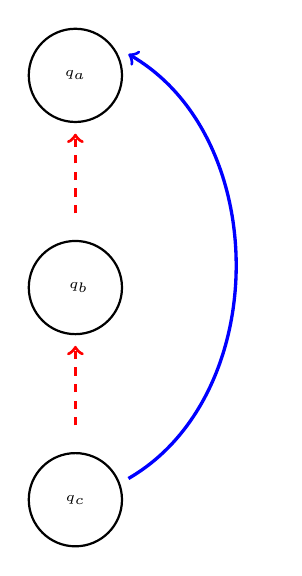
\begin{tikzpicture}[scale=\textwidth/18cm,samples=200]
%%% The nodes represents the k query in the first round
% \draw[very thick] (-1,6)  -- (13,6) -- (13,3) -- (-1,3) -- (-1,6);
% \draw[black] (-2.5, 4) circle (0pt) node [anchor=south]{\textbf{line 4:}};
\draw[thick] (2, 12.1) circle (25pt) node
% node[label={above: \small{iteration 1:}}] 
{\tiny{$q_a$}} ;
\draw[thick] (2, 8.1) circle (25pt) node
{\tiny{ $q_b$}};
 \draw[thick] (2, 4.1) circle (25pt) node 
{\tiny{$q_c$}};
% \filldraw[black] (-2.5, 0) circle (0pt) node [anchor=south]{\textbf{line 7:}};
% \draw[thick] (6, 0) circle (25pt) node {\tiny{$q_4^7$}};
\draw[very thick,->, red, dashed] (2, 5.5)  -- (2, 7.0) ;
\draw[very thick,->, red, dashed] (2, 9.5)  to  (2, 11.0) ;
\draw[very thick,->, blue] (3, 4.5)  to   [out=30,in=-30] (3, 12.5) ;
\end{tikzpicture}
\caption{}
    \end{centering}
    \end{subfigure}
    \begin{subfigure}{0.5\textwidth}
    \begin{centering}
    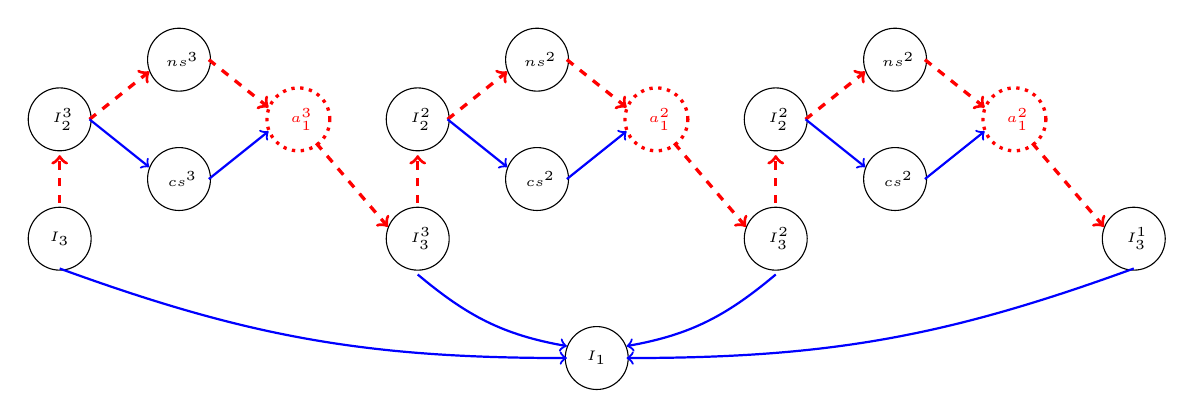
\begin{tikzpicture}[scale=\textwidth/16cm,samples=200]
%%% The nodes represents the k query in the first round
% \draw[very thick] (-1,6)  -- (13,6) -- (13,3) -- (-1,3) -- (-1,6);
% \draw[black] (-2.5, 4) circle (0pt) node [anchor=south]{\textbf{line 4:}};
% \draw[thick] (1, 1.1) circle (25pt) node
% % node[label={above: \small{iteration 1:}}] 
% {\tiny{$q_1^{(5,1)}$}} ;
% \draw[] (2, 5.1) circle (15pt) node
% {\tiny{ $I_1$}};
\draw[] (19, 7.1) circle (15pt) node
{\tiny{ $I_3^{1}$}};
% \draw[thick] (8, 11.1) circle (15pt) node
% {\tiny{ $x_{1}^{1}$}};
% \draw[thick] (10, 10.1) circle (15pt) node
% {\tiny{ $x_{2}^{1}$}};
% \draw[] (8, 9.1) circle (15pt) node
% {\tiny{ $x_{3}^{1}$}};
% \draw[] (8, 7.1) circle (15pt) node
% {\tiny{ $I_{2}^{1}$}};
\draw[very thick, red, dotted] (17, 9.1) circle (15pt) node
{\tiny{ $a_{1}^{2}$}};
\draw[] (15, 10.1) circle (15pt) node
{\tiny{ $ns^{2}$}};
\draw[] (15, 8.1) circle (15pt) node
{\tiny{ $cs^{2}$}};
\draw[] (13, 9.1) circle (15pt) node
{\tiny{ $I_{2}^{2}$}};
\draw[] (13, 7.1) circle (15pt) node
{\tiny{ $I_3^{2}$}};
% \draw[thick] (10, 8.1) circle (15pt) node
% {\tiny{ $x_{1}^{2}$}};
% \draw[thick] (12, 7.1) circle (15pt) node
% {\tiny{ $x_{2}^{2}$}};
% \draw[] (10, 8.1) circle (15pt) node
% {\tiny{ $x_{3}^{2}$}};
% \draw[] (9, 10.1) circle (15pt) node
% {\tiny{ $I_{2}^{1}$}};
% \draw[thick] (12, 5.1) circle (15pt) node
% {\tiny{ $x_1^{3}$}};
\draw[very thick, red, dotted] (11, 9.1) circle (15pt) node
{\tiny{ $a_{1}^{2}$}};
\draw[] (9, 10.1) circle (15pt) node
{\tiny{ $ns^{2}$}};
\draw[] (9, 8.1) circle (15pt) node
{\tiny{ $cs^{2}$}};
\draw[] (7, 9.1) circle (15pt) node
{\tiny{ $I_{2}^{2}$}};
\draw[] (7, 7.1) circle (15pt) node
{\tiny{ $I_3^{3}$}};
%%%%%%%%%%%%%%%%%%%%%
\draw[very thick, red, dotted] (5, 9.1) circle (15pt) node
{\tiny{ $a_{1}^{3}$}};
\draw[] (3, 10.1) circle (15pt) node
{\tiny{ $ns^{3}$}};
\draw[] (3, 8.1) circle (15pt) node
{\tiny{ $cs^{3}$}};
\draw[] (1, 9.1) circle (15pt) node
{\tiny{ $I_{2}^{3}$}};
 \draw[] (1, 7.1) circle (15pt) node 
{\tiny{$I_3$}};
 \draw[] (10, 5.1) circle (15pt) node 
{\tiny{$I_1$}};
% \filldraw[black] (-2.5, 0) circle (0pt) node [anchor=south]{\textbf{line 7:}};
% \draw[thick] (6, 0) circle (15pt) node {\tiny{$l_1$}};
 \draw[very thick,->, red, dashed] (1, 7.7)  -- (1, 8.5) ;
 \draw[very thick,->, red, dashed] (1.5,9.1)  -- (2.5, 9.9) ;
 \draw[thick,->, blue] (1.5,9.1)  -- (2.5, 8.3) ;
 \draw[very thick,->, red, dashed] (3.5,10.1)  -- (4.5, 9.3) ;
 \draw[thick,->, blue] (3.5,8.1)  -- (4.5, 8.9) ;
 \draw[very thick,->, red, dashed] (5.3,8.7)  -- (6.5, 7.3) ;
 %%%%%%%%%%
  \draw[very thick,->, red, dashed] (7, 7.7)  -- (7, 8.5) ;
 \draw[very thick,->, red, dashed] (7.5,9.1)  -- (8.5, 9.9) ;
 \draw[thick,->, blue] (7.5,9.1)  -- (8.5, 8.3) ;
 \draw[very thick,->, red, dashed] (9.5,10.1)  -- (10.5, 9.3) ;
 \draw[thick,->, blue] (9.5,8.1)  -- (10.5, 8.9) ;
 \draw[very thick,->, red, dashed] (11.3,8.7)  -- (12.5, 7.3) ;
 %%%
  \draw[very thick,->, red, dashed] (13, 7.7)  -- (13, 8.5) ;
 \draw[very thick,->, red, dashed] (13.5,9.1)  -- (14.5, 9.9) ;
 \draw[thick,->, blue] (13.5,9.1)  -- (14.5, 8.3) ;
 \draw[very thick,->, red, dashed] (15.5,10.1)  -- (16.5, 9.3) ;
 \draw[thick,->, blue] (15.5,8.1)  -- (16.5, 8.9) ;
 \draw[very thick,->, red, dashed] (17.3,8.7)  -- (18.5, 7.3) ;
 %%%%
 \draw[thick,->, blue] (1,6.6)   to   [out=-20,in=180] (9.5, 5.1) ;
 \draw[thick,->, blue] (7,6.5)  to   [out=-40,in=170] (9.5, 5.3) ;
 \draw[thick,->, blue] (13,6.5)   to   [out=-140,in=10] (10.5, 5.3) ;
 \draw[thick,->, blue] (19,6.6)  to   [out=-160,in=0] (10.5, 5.1) ;
\end{tikzpicture}
    \caption{}
    \end{centering}
    \end{subfigure}
    \vspace{-0.4cm}
    \caption{(a) The query-based dependency graph for multiple round example (b) The SSA variable-based weighted dependency graph for the same example, the node in red dashed circle is weighted.}
    \vspace{-0.2cm}
    \label{fig:multi_graphs}
\end{figure}
%
%
% \begin{figure}
% \begin{tikzpicture}[scale=\textwidth/25cm,samples=200]
% %%% The nodes represents the k query in the first round
% \filldraw[black] (0, 4) circle (5pt) node [anchor=south]{$q^{3, []}_{1}(0, 3)$};
% \filldraw[black] (12, 4) circle (5pt) node [anchor=south]{$q^{3, []}_{1}(2, 3)$};
% \draw[very thick, ->, red] (12, 4)  to [out=150,in=30] (0, 4.1) ;
% \end{tikzpicture}
%     \caption{A query-based dependency graph for multi round algorithm}
%     \label{fig:multi-round-graph}
% \end{figure}
% \begin{figure}
% \begin{tikzpicture}[scale=\textwidth/25cm,samples=200]
% %%% The nodes represents the k query in the first round
% \filldraw[black] (0, 4) circle (5pt) node [anchor=south]{$q^{3, []}_{1}(0, 3)$};
% \filldraw[black] (6, 3) circle (5pt) node [anchor=north]{$q^{3, []}_{1}(1, 3)$};
% \filldraw[black] (12, 4) circle (5pt) node [anchor=south]{$q^{3, []}_{1}(2, 3)$};
% \filldraw[black] (6, 0) circle (5pt) node [anchor=north]{$q^{6, []}_{2}([1, 0, 1])$};
% \draw[very thick, ->, blue] (12, 4)  to [out=150,in=30] (0, 4.1) ;
% % \draw[very thick,->] (3, 4)  -- (0, 4) ;
% % \draw[very thick,->] (0, 0)  -- (6, 2) ;
% %%%%%% The edges represents their dependency relations GROUP 2
% %
% \draw[very thick,->, red]  (12, 4) to [out=150,in=60] (6.1, 3) ;
% \draw[very thick,->, red] (6, 3)  to [out=120,in=30] (0, 3.95) ;
% % %
% %%%%%% The edges represents their dependency relations GROUP 4
% % \draw[very thick,->] (0, 0)  -- (6, 2) ;
% % \draw[very thick,->] (12, 2)  -- (8.1, 2) ;
% \draw[very thick,->, blue] (6, 0)  -- (6, 2.9) ;
% \draw[very thick,->, red] (6, 0)  -- (12, 3.9) ;
% \draw[very thick,->, blue] (6, 0)  -- (0, 3.9) ;
% \end{tikzpicture}
%     \caption{A query-based dependency graph for multi round algorithm}
%     \label{fig:multi-round-graph}
% \end{figure}
%
%
% Using \ADAPTSYSTEM, we first generate a global list $G$ from an empty list $[]$ and empty whlemap $\emptyset$.
%  \[[]; \emptyset; MR^{ssa} \to G; w  \land w = \emptyset\].
%  \[G_{k=2} = \left[
%   {I_1}^{(1,\emptyset)} , {I_3}^{(2,[2:1])} , {p_1}^{(3,[2:1])} , {a_1}^{(4,[2:1])} ,{I_2}^{(5,[2:1])} ,  {I_3}^{(2,[2:2])} , {p_1}^{(3,[2:2])} , {a_1}^{(4,[2:2])} ,{I_2}^{(5,[2:2])} , {I_3}^{(2,\emptyset)}   \right] \]
%   We denote $I_1^{1}$ short for ${I_1}^{(1,\emptyset)}$ and ${I_3}^{(2,1)}$ short for ${I_3}^{(2,[2:1])}$, where the label $(2, 1)$ represents at line number $2$ and in the $1$ st iteration. 
% \[
% M =  \left[ \begin{matrix}
%   I_1^{1} & I_3^{(2,1)} & p_1^{(3,1)} & a_1^{(4,1)} &I_2^{(5,1)}  & I_3^{(2,2)} & p_1^{(3,2)} & a_1^{(4,2)} & I_2^{(5,2)} & I_3^{2}\\
%   0 & 0 & 0 & 0 & 0 & 0 & 0 &0 &0&0  \\
%  1 & 0 & 0 & 0 & 0 & 0 & 0&0&0&0\\
%  0 & 0 & 0 & 0 & 0 & 0& 0& 0 &0&0\\
%  0 & 1 & 0 & 0 & 0 & 0 & 0& 0&0&0\\
%  0 & 1 & 1 & 1 & 0 & 0 & 0 & 0&0 &0\\
%  1 & 0 & 0 & 0 & 1 & 0 & 0& 0&0&0\\
%  0 & 0 & 0 & 0 & 0 & 0 & 0& 0&0&0\\
%  0 & 0 & 0 & 0 & 0 & 1 & 0& 0&0&0\\
%  0 & 0 & 0 & 0 & 0 & 1 & 1 & 1 &0 &0\\
% 1 & 0 & 0 & 0 & 0 & 0 & 0 & 0 &1&0 \\
%  \end{matrix} \right] 
% ~ , V = \left [ \begin{matrix}
% I_1^{1} &  0 \\
% I_3^{(2,1)} &  0 \\
% p_1^{(3,1)} & 0 \\
% a_1^{(4,1)} &  1 \\
% I_2^{(5,1)} & 0 \\
% I_3^{(2,2)} & 0 \\
% p_1^{(3,2)} &  0 \\
% a_1^{(4,2)} & 1 \\
% I_2^{(5,2)} & 0 \\
% I_3^{2} & 0 \\
% \end{matrix} \right ]
% \]
%
%
%
%\begin{figure}
% \begin{center}
% %
% \begin{tikzpicture}[scale=\textwidth/17cm,samples=200]
% %%% The nodes represents the k query in the first round
% \filldraw[red] (0, 3) circle (2pt) node [anchor=south]{$a_1^{(4,1)}$};
% \filldraw[black] (3, 4) circle (2pt) node [anchor=south]{$p_1^{(3,1)}$};
% % \filldraw[black] (6, 2) circle (2pt) node [anchor=south]{$q^4_3$};
% \filldraw[black] (6, 4) circle (2pt) node [anchor=south]{$p_1^{(3,2)}$};
% \filldraw[black] (8, 3) circle (2pt) node [anchor=south]{$I_3^{(2,1)}$};
% %%%%%% The nodes represents the n^k queries in the second round
% \filldraw[red] (0, 2) circle (2pt) node [anchor=north]{$a_1^{(4,2)}$};
% \filldraw[black] (3, 0) circle (2pt) node [anchor=north]{$I_2^{(5,1)}$};
% % \filldraw[black] (6, 0) circle (2pt) node [anchor=north]{$q^{3, 7}_{k+1}$};
% \filldraw[black] (6, 0) circle (2pt) node [anchor=north]{$I_2^{(5,2)}$};
% \filldraw[black] (8, 1) circle (2pt) node [anchor=north]{$I_3^{(2,3)}$};
% \filldraw[black] (8, 2) circle (2pt) node [anchor=south]{$I_3^{(2,2)}$};
% \filldraw[black] (12, 2) circle (2pt) node [anchor=south]{$I_1^{1}$};
% %%%%%The edges between a and I
% %%%%% (a1(4,1), I3(2,1))
% \draw[very thick, ->] (0, 3)  -- (7.9, 3) ;
% %%%%% (a1(4,2), I3(2,2))
% \draw[very thick, ->] (0, 2)  -- (7.9, 2) ;
% %%%%%% The edges represents their dependency relations GROUP between I3 and I1
% \draw[very thick,<-] (12, 2)  -- (8, 2) ;
% \draw[very thick,->] (8, 2) -- (3.1, 0) ;
% %
% \draw[very thick,<-] (12, 2)  -- (8, 1) ;
% \draw[very thick,->] (8, 1) -- (6.1, 0) ;
% %
% \draw[very thick,<-] (12, 2)  -- (8, 3) ;
% %
% %%%%%% The edges represents their dependency relations GROUP between I2 and others
% %%%%%% The edges represents their dependency relations GROUP between I2(5,1) and others
% \draw[very thick, ->] (3, 0)  -- (0, 2.9) ;
% \draw[very thick, ->] (3, 0)  -- (3, 3.9) ;
% \draw[very thick, ->] (3, 0)  -- (7.9, 2.9) ;
% %%%%%% The edges represents their dependency relations GROUP between I2(5,2) and others
% \draw[very thick, ->] (6, 0)  -- (0, 1.9) ;
% \draw[very thick, ->] (6, 0)  -- (6, 3.9) ;
% \draw[very thick, ->] (6, 0)  -- (7.9, 1.9) ;
% %%%% The longest path representing the adaptivity
% \draw[ultra thick, red, ->, dashed] (0, 2) -- (7.9, 2);
% \draw[ultra thick, red, ->, dashed] (8, 2) -- (3.1, 0);
% \draw[ultra thick, red, ->, dashed] (3, 0)  -- (0, 2.9);
% \end{tikzpicture}
% \end{center}
%     \caption{the variable dependency graph for multi round algorithm}
%     \label{fig:multi-round-graph-ssa}
% \end{figure}
%
% The adaptivity is 1 computed from the graph.
% The query-based dependency graph is a subgraph of the variable dependency graph for multi round algorithm.
%

\section{ Over-approximation Algorithm}
\label{sec:adapt-example-over}

Our algorithm comes across an over-approximation on the estimation due to its path-insensitive nature. It occurs when the control flow can be decided in a particular way in front of conditional branches, while the static analysis fails to witness. 

We use one example to show the over-approximation, Figure~\ref{fig:overappr_example}(a). This example is the variant of the multiple rounds strategy, 
we call it a multiple rounds odd iteration algorithm. In this algorithm, at every iteration, a query $q(b+\chi[i])$ based on previous query results stored in $b$ is asked by the analyst like in the multiple rounds strategy. The difference is that only the query answers from odd iterations ($i =1,3, 5$) are added to $b$. 
  Because the execution trace only updates $b$ using the query answers at odd iterations, so the answers from even iterations do not affect the queries at odd iterations. From the query-based dependency graph in Figure~\ref{fig:overappr_example}(b), we can see that there is no edge from queries at odd iterations (such as $q_1,q_3,q_5$) to queries at even iteration(such as $q_2,q_4$). The longest path is dashed with a length $3$.  However, {\ADAPTSYSTEM} fails to realize that odd iteration will always execute then branch and even iteration means else branch, so its dependency graph considers both branches for every iteration. In this sense, the dependency graph by {\ADAPTSYSTEM} is similar to the one in the multiple rounds strategy. We show the estimated graph in Figure~\ref{fig:overappr_example}(c). The estimated upper bound is then, $5$, instead of $3$. 
%

{ 
\begin{figure}
\centering
    \begin{subfigure}{0.3\textwidth}
\centering
    $
    \begin{array}{l}
      \clabel{ \assign{b}{0}}^{1} ; \\
      \clabel{ \assign{i}{1}}^{1} ; \\
      \eloop ~ \clabel{5}^3 ~ \edo ~ \\
      \quad  \clabel{\assign{x}{q(b+\chi[i-1])}}^{4};\\
      \quad \eif ( [(i \% 2 ==1 )]^{5} \\
      \quad \quad,\clabel{\assign{b}{b+x}}^{6}\\
      \quad \quad, \clabel{\eskip}^{7});\\
     \quad \clabel{\assign{i}{i+1}}^{8}  
 \end{array}
 $
 \caption{}
    \end{subfigure}
%
\begin{subfigure}{0.3\textwidth}
\centering
    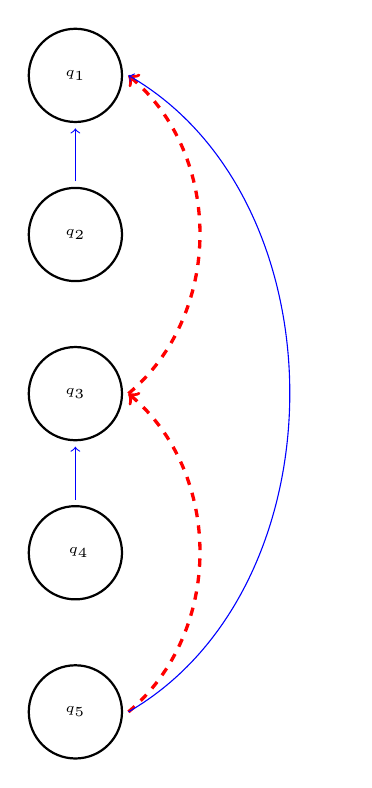
\begin{tikzpicture}[scale=\textwidth/18cm,samples=200]
%%% The nodes represents the k query in the first round
% \draw[very thick] (-1,6)  -- (13,6) -- (13,3) -- (-1,3) -- (-1,6);
% \draw[black] (-2.5, 4) circle (0pt) node [anchor=south]{\textbf{line 4:}};
\draw[thick] (6, 14.1) circle (25pt) node
{\tiny{$q_1$}} ;
\draw[thick] (6, 11.1) circle (25pt) node
{\tiny{$q_2$}} ;
\draw[thick] (6, 8.1) circle (25pt) node
{\tiny{$q_3$}} ;
\draw[thick] (6, 5.1) circle (25pt) node
{\tiny{ $q_4$}};
 \draw[thick] (6, 2.1) circle (25pt) node 
{\tiny{$q_5$}};
% \filldraw[black] (-2.5, 0) circle (0pt) node [anchor=south]{\textbf{line 7:}};
% \draw[thick] (6, 0) circle (25pt) node {\tiny{$q_4^7$}};
\draw[very thick,->, red, dashed] (7, 2.1)  to   [out=40,in=-40] (7, 8.1) ;
\draw[very thick,->, red, dashed] (7, 8.1)  to   [out=40,in=-40] (7, 14.1) ;
\draw[->, blue] (7, 2.1)  to   [out=30,in=-30]  (7, 14.1) ;
\draw[->, blue] (6, 6.1)  to    (6, 7.1) ;
\draw[->, blue] (6, 12.1)  to    (6, 13.1) ;
% \draw[very thick,->, red, dashed] (2, 9.5)  to  (2, 11.0) ;
% \draw[very thick,->, blue] (3, 4.5)  to   [out=10,in=10] (3, 12.5) ;
\end{tikzpicture}
\caption{}
    \end{subfigure}
%
\begin{subfigure}{0.3\textwidth}
\centering
    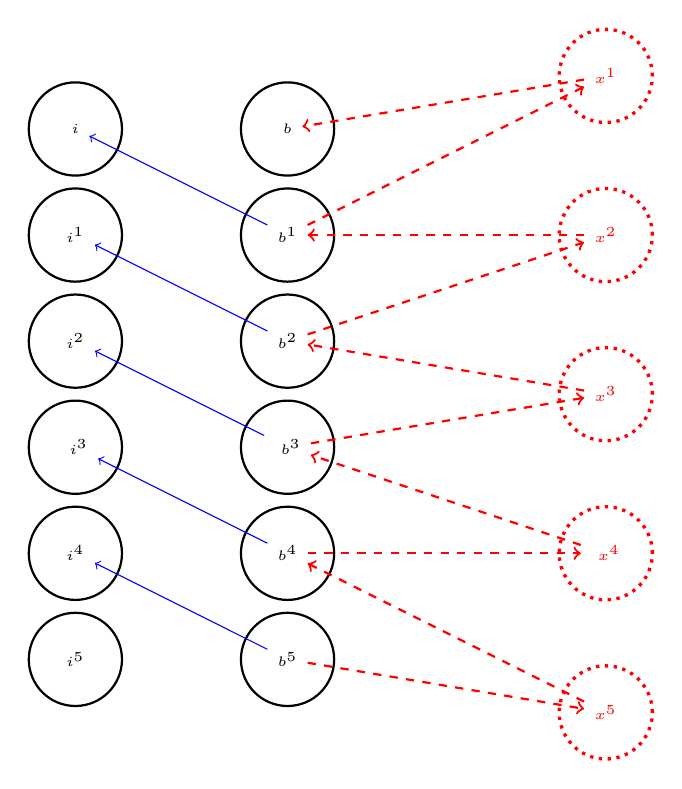
\begin{tikzpicture}[scale=\textwidth/18cm,samples=200]
%%% The nodes represents the k query in the first round
% \draw[very thick] (-1,6)  -- (13,6) -- (13,3) -- (-1,3) -- (-1,6);
% \draw[black] (-2.5, 4) circle (0pt) node [anchor=south]{\textbf{line 4:}};
\draw[thick] (0, 14.1) circle (25pt) node(i)
{\tiny{$i$}} ;
\draw[thick] (0, 12.1) circle (25pt) node(i1)
{\tiny{$i^1$}} ;
\draw[thick] (0, 10.1) circle (25pt) node(i2)
{\tiny{$i^2$}} ;
\draw[thick] (0, 8.1) circle (25pt) node (i3)
{\tiny{ $i^3$}};
 \draw[thick] (0, 6.1) circle (25pt) node (i4)
{\tiny{$i^4$}};
 \draw[thick] (0, 4.1) circle (25pt) node (i5)
{\tiny{$i^5$}};
%
\draw[thick] (4, 14.1) circle (25pt) node(b)
{\tiny{$b$}} ;
\draw[thick] (4, 12.1) circle (25pt) node
(b1){\tiny{$b^1$}} ;
\draw[thick] (4, 10.1) circle (25pt) node (b2)
{\tiny{$b^2$}} ;
\draw[thick] (4, 8.1) circle (25pt) node (b3)
{\tiny{ $b^3$}};
 \draw[thick] (4, 6.1) circle (25pt) node (b4)
{\tiny{$b^4$}};
 \draw[thick] (4, 4.1) circle (25pt) node (b5)
{\tiny{$b^5$}};
%
\draw[very thick, red, dotted] (10, 15.1) circle (25pt) node (x1)
{\tiny{$x^1$}} ;
\draw[very thick, red, dotted] (10, 12.1) circle (25pt) node (x2)
{\tiny{$x^2$}} ;
\draw[very thick, red, dotted] (10, 9.1) circle (25pt) node(x3)
{\tiny{$x^3$}} ;
\draw[very thick, red, dotted] (10, 6.1) circle (25pt) node (x4)
{\tiny{ $x^4$}};
 \draw[very thick, red, dotted] (10, 3.1) circle (25pt) node (x5)
{\tiny{$x^5$}};
%Dependency between b and i
\draw[->, blue] (b1)  to    (i) ;
\draw[->, blue] (b2)  to    (i1) ;
\draw[->, blue] (b3)  to    (i2) ;
\draw[->, blue] (b4)  to    (i3) ;
\draw[->, blue] (b5)  to    (i4) ;
%Dependency between b and x
\draw[->, thick, red, dashed] (b1)  to    (x1) ;
\draw[->, thick, red, dashed] (b2)  to    (x2) ;
\draw[->, thick, red, dashed] (b3)  to    (x3) ;
\draw[->, thick, red, dashed] (b4)  to    (x4) ;
\draw[->, thick, red, dashed] (b5)  to    (x5) ;
%Dependency between x and b
\draw[->, thick, red, dashed] (x1)  to    (b) ;
\draw[->, thick, red, dashed] (x2)  to    (b1) ;
\draw[->, thick, red, dashed] (x3)  to    (b2) ;
\draw[->, thick, red, dashed] (x4)  to    (b3) ;
\draw[->, thick, red, dashed] (x5)  to    (b4) ;
% \filldraw[black] (-2.5, 0) circle (0pt) node [anchor=south]{\textbf{line 7:}};
% \draw[thick] (6, 0) circle (25pt) node {\tiny{$q_4^7$}};
% \draw[very thick,->, red, dashed] (7, 2.1)  to   [out=40,in=-40] (7, 8.1) ;
% \draw[very thick,->, red, dashed] (7, 8.1)  to   [out=40,in=-40] (7, 14.1) ;
% \draw[very thick,->, blue] (7, 2.1)  to   [out=30,in=-30]  (7, 14.1) ;
% \draw[very thick,->, blue] (6, 6.1)  to    (6, 7.1) ;
% \draw[very thick,->, blue] (6, 12.1)  to    (6, 13.1) ;
% \draw[very thick,->, red, dashed] (2, 9.5)  to  (2, 11.0) ;
% \draw[very thick,->, blue] (3, 4.5)  to   [out=10,in=10] (3, 12.5) ;
\end{tikzpicture}
\caption{}
    \end{subfigure}
    \vspace{-0.3cm}
\caption{(a) The labeled program implementing multiple round odd iteration example (b) The query-based dependency graph for the example (c) The SSA variable-based weighted dependency graph for the same example.}
    \label{fig:overappr_example}
    \vspace{-0.5cm}
\end{figure}
}
%
%
% By assuming a specific database $D = [[1], [0], [1], [1]]$,
% $q_1$ is counting query, and $q_2(x)$ is returning the $x^{th}$ row of the data base, the execution trace is generated as:
% \[
%  t_{mr} = \left\{
% q_1^{1, []}
% \right \}
% \]
% % $\config{[], MR(2), D, []>} \to^{*} 
% % \config{[j \to 3, a \to [1, 0, 1], l \to 1], D, \eskip, []>}$
% % \\
% Then we have the dependency graph generated as following, with the graph shown in Figure \ref{fig:multi-round-graph}.
% \\
% $V = \left\{
% q_1^{1, []}
% \right \}$
% \\
% $E = \left \{
% \right\}$
% \\
% Then we have the adaptivity calculated from the graph as follows:
% \[
% \begin{array}{ll}
% A^*(c, D, m, w) & = \max\limits_{q(v)^{(l,w)},q(v')^{(l',w')} \in V }\{ |p(q(v)^{(l,w)}, q(v')^{(l',w')} )| \}\\
% & = 0
% \end{array}
% \]
% %
% % 
% Using \ADAPTSYSTEM, we first generate a global list $G$ from an empty list $[]$ and empty whlemap $\emptyset$.
%  \[
%  []; \emptyset; MR^{ssa} \to G; w  \land w = \emptyset
%  \].
%  %
%  \[
%  G = \left[  x_1^{1, []}, x_2^{3, []}   \right] 
%  \]
%  %
%  %
% \[
% M =  \left[ 
% \begin{matrix}
%   & x_1^{1, []} & x_2^{3, []}\\
%  x_1^{1, []}  & 0 & 0   \\
%  x_2^{3, []} & 1 & 0 
%  \end{matrix} \right] 
% ~ , V = \left [ \begin{matrix}
%  x_1^{1, []} &  1 \\
% x_2^{3, []} &  1
% \end{matrix} \right ]
% \]
% %
% %
% %
% \begin{figure}
% \centering
% \begin{subfigure}[b]{0.3\textwidth}
% \centering
% \begin{tikzpicture}[scale=\textwidth/25cm,samples=200]
% %%% The nodes represents the k query in the first round
% \filldraw[black] (0, 4) circle (5pt) node [anchor=south]{$q_1^{1, []}$};
% % \filldraw[black] (12, 4) circle (5pt) node [anchor=south]{$q_2^{3}$};
% % \draw[very thick, ->, red] (12, 4)  to [out=150,in=30] (0, 4.1) ;
% \end{tikzpicture}
%     \caption{A query-based dependency graph for  over-approximation algorithm}
%     \label{fig:over-approx-graph}
% \end{subfigure}
% \hspace{2cm}
% \begin{subfigure}[b]{0.3\textwidth}
% \centering
% \begin{tikzpicture}[scale=\textwidth/17cm,samples=200]
% %%% The nodes represents the k query in the first round
% \filldraw[red] (0, 4) circle (5pt) node [anchor=south]{$x_1^{1, []}$};
% \filldraw[red] (12, 4) circle (5pt) node [anchor=south]{$x_2^{3, []}$};
% \draw[very thick, ->, red] (12, 4)  to [out=150,in=30] (0, 4.1) ;
% \end{tikzpicture}
% \caption{the variable dependency graph for over-approximation algorithm}
%     \label{fig:over-approx-graph-ssa}
% \end{subfigure}
% \end{figure}
%
% \begin{figure}
% \begin{center}
% %
% \begin{tikzpicture}[scale=\textwidth/17cm,samples=200]
% %%% The nodes represents the k query in the first round
% \filldraw[black] (0, 4) circle (5pt) node [anchor=south]{$x_1^{1}$};
% \filldraw[black] (12, 4) circle (5pt) node [anchor=south]{$x_2^{3}$};
% \draw[very thick, ->, red] (12, 4)  to [out=150,in=30] (0, 4.1) ;
% \end{tikzpicture}
% \end{center}
%     \caption{the variable dependency graph for over-approximation algorithm}
%     \label{fig:over-approx-graph-ssa}
% \end{figure}
%
% The adaptivity is 1 computed from the graph.
% The query-based dependency graph is a subgraph of the variable dependency graph for multi round algorithm.